\section{Change of object's location over time}
\label{sec-change-location}

\textbf{Created by:} Arkopaul Sarkar \\
\textbf{Modified by:} Arkopaul Sarkar \\

\subsection*{Scenario Objective}

This scenario illustrates how to represent the change in an object's physical location over time using the IOF/BFO ontology framework. It focuses on:
\begin{itemize}
    \item Emphasizing physical locations as sites and their association with spatial regions.
    \item Capturing actual movements of objects between existing locations (does not express any future plan or schedule of movement).
    \item \textbf{Temporal focus:} Associating specific temporal instants with the object's presence at particular locations.
\end{itemize}

\subsection*{General Pattern Description}
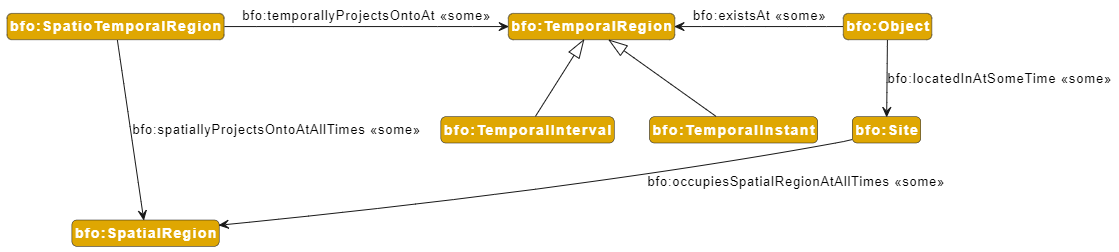
\includegraphics[scale=0.38]{scenarios/location-change/images/change-location-general.png}


\subsubsection*{Use Case: Freight Train Location Change} 
A freight train operated by BNSF Railway hauls coal from Powder River Basin, Wyoming, to the Port of Long Beach in California. It was located at Powder River Basin station at 11:00 AM on Wednesday and then at Long Beach station at midnight on Thursday.

\subsubsection*{Use-Case Pattern Description}

\begin{itemize}
    \item The train \texttt{ns1:freight-train} is located at (\texttt{bfo:locatedInAtSomeTime}) two different locations: \texttt{ns1:powder-river-basin} and \texttt{ns1:long-beach-port}, both of which are instances of \texttt{bfo:site}.
    \item Two separate instances of \texttt{bfo:SpatialRegion}: \texttt{ns1:spatial-region-powder-river-basin} and \texttt{ns1:spatial-region-long-beach}.
    \item The sites are linked to the spatial regions by \texttt{occupiesSpatialRegionAtAllTimes}.
    \item Temporal instants are linked to the sites, but the actual clock times are omitted for brevity.
\end{itemize}


\subsubsection*{Use-Case Diagram}
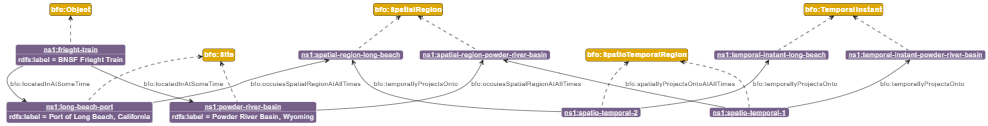
\includegraphics[scale=0.45]{scenarios/location-change/images/change-location-usecase1.png}

\subsubsection*{Use-Case Example Data}

\begin{tabularx}{\textwidth}{|X|l|X|X|X|}
\hline
Train Number & Source & Destination & Departure Time & Arrival Time \\
\hline
1            & Powder River Basin & Long Beach      & 11:00 AM      & Midnight       \\
2            & Example Source     & Example Dest    & 10:00 AM      & 2:00 PM        \\
3            & Example Source 2   & Example Dest 2  & 8:00 AM       & 4:00 PM        \\
\hline
\end{tabularx}

\subsubsection*{Data Mapping Description}

\begin{verbatim}
INSERT DATA {
    <http://example.org/ns1:freight-train> a <http://example.org/bfo:Entity>;
    <http://example.org/ns1:freight-train> <http://example.org/bfo:locatedInAtSomeTime> 
        <http://example.org/ns1:powder-river-basin>.
}
\end{verbatim}

\subsubsection*{Data Validation}